% ============================================================
%  Template Presentazione Tesi — versione pulita
%  Compilare con: pdflatex > pdflatex
%  Oppure carica su Overleaf e premi "Recompile".
% ============================================================

\documentclass[aspectratio=169]{beamer}

% ── Tema base ───────────────────────────────────────────────
\usetheme{Madrid}
\usecolortheme{default}

% ── Palette colori sobria (blu/grigio accademico) ───────────
\definecolor{thesisBlue}{HTML}{1F3864}
\definecolor{thesisBlueLight}{HTML}{2E5090}
\definecolor{thesisGray}{HTML}{4D4D4D}
\definecolor{thesisBg}{HTML}{F5F5F5}
\definecolor{thesisAccent}{HTML}{8C1D1D}   % rosso scuro per gli alert, usato con parsimonia

\setbeamercolor{palette primary}{bg=thesisBlue, fg=white}
\setbeamercolor{palette secondary}{bg=thesisBlueLight, fg=white}
\setbeamercolor{palette tertiary}{bg=thesisGray, fg=white}
\setbeamercolor{structure}{fg=thesisBlue}
\setbeamercolor{block title}{bg=thesisBlue, fg=white}
\setbeamercolor{block body}{bg=thesisBg, fg=black}
\setbeamercolor{alerted text}{fg=thesisAccent}

% ── Pacchetti ───────────────────────────────────────────────
\usepackage[T1]{fontenc}
\usepackage[utf8]{inputenc}
\usepackage[italian]{babel}
\usepackage{lmodern}
\usepackage{listings}
\usepackage{xcolor}
\usepackage{graphicx}
\usepackage{tikz}
\usepackage{booktabs}
\usetikzlibrary{positioning}

% ── Stile listings (per eventuale codice) ───────────────────
\lstset{
  basicstyle=\ttfamily\small,
  keywordstyle=\color{thesisBlue}\bfseries,
  stringstyle=\color{green!40!black},
  commentstyle=\color{gray}\itshape,
  frame=single,
  rulecolor=\color{thesisBlue!40},
  xleftmargin=1em,
  xrightmargin=1em,
  numbers=none,
  breaklines=true,
  showstringspaces=false,
}

% ── Metadati (da compilare) ──────────────────────────────────
\title{Un linguaggio per domarli tutti: applicazioni full stack con librerie native in Kotlin Multiplatform}
\author{Sohaib Ouakani}
\institute{
    Corso di Laurea in Ingegneria e Scienze informatiche \\
    Relatore: Prof. Danilo Pianini \\
    Correlatori: Dott. Angela Cortecchia, Ing. Valter Venusti
}
\date{A.A. 2025/2026}

\setbeamertemplate{footline}[frame number]
\setbeamertemplate{navigation symbols}{}


% ============================================================
\begin{document}

% ── SLIDE TITOLO ─────────────────────────────────────────────
\begin{frame}
  \titlepage
\end{frame}

% ── INDICE ───────────────────────────────────────────────────
\begin{frame}{Indice}
  \tableofcontents
\end{frame}


% ============================================================
\section{Contesto}
% ============================================================

\begin{frame}{Contesto: stack software eterogeneo}
  \begin{columns}
    \column{0.55\textwidth}
      \begin{itemize}
        \item Stack industriali spesso eterogenei
        \item Librerie di standard tecnici scritte in linguaggi nativi
        \item Risultato: duplicazione di codice, complessità, manutenzione difficile
      \end{itemize}
    \column{0.4\textwidth}
      \begin{block}{Problema}
        Si può usare un solo linguaggio per l'intero applicativo, mantenendo l'accesso a librerie native di dominio?
      \end{block}
  \end{columns}
\end{frame}


% ============================================================
\section{Approcci esistenti}
% ============================================================

\begin{frame}{Approcci esistenti}
  \begin{columns}
    \column{0.55\textwidth}
      \begin{itemize}
        \item Node.js: molto popolare, ma interazione con il nativo complessa
        \item Linguaggi fullstack popolari richiedono spesso codice in altri linguaggi
      \end{itemize}
    \column{0.4\textwidth}
      \begin{alertblock}{Limite principale}
        Serve codice legante in C per interagire con librerie native
      \end{alertblock}
  \end{columns}
\end{frame}


% ============================================================
\section{La Soluzione Proposta}
% ============================================================

\begin{frame}{La soluzione}
  \begin{block}{Kotlin Multiplatform + CInterop}
    Applicazione fullstack multipiattaforma in Kotlin, con accesso diretto al nativo tramite CInterop
  \end{block}
  \vspace{0.6em}
  \begin{itemize}
    \item Un solo linguaggio per tutto lo stack: Kotlin
    \item Interfaccia diretta con C tramite CInterop
    \item Nessun layer di astrazione intermedio
  \end{itemize}
\end{frame}


% ============================================================
\section{Standard FMI e formato FMU (Background)}
% ============================================================

\begin{frame}{Standard FMI e formato FMU}
  \begin{columns}
    \column{0.55\textwidth}
      \begin{itemize}
        \item FMI: standard per lo scambio di modelli di simulazione, con interfaccia C
        \item FMU: archivio zip con modello e metadati, secondo lo standard FMI
      \end{itemize}
    \column{0.4\textwidth}
      \begin{block}{Perché sono rilevanti}
        Caso di studio per validare l'approccio Kotlin fullstack in ambito industriale
      \end{block}
  \end{columns}
\end{frame}


% ============================================================
\section{Architettura}
% ============================================================

\begin{frame}{Architettura del sistema}
  \begin{columns}
    \column{0.6\textwidth}
      \begin{figure}
          \centering
          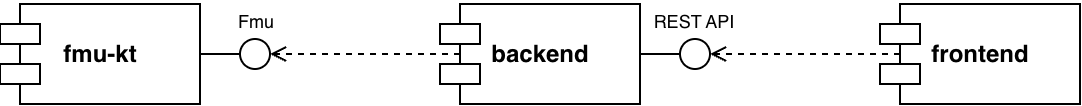
\includegraphics[width=\textwidth]{images/diagramma-tirocinio.png}
          \caption{Architettura generale del sistema.}
          \label{fig:architettura}
      \end{figure}
    \column{0.38\textwidth}
      \begin{block}{Linguaggi}
        \begin{itemize}
          \item Frontend: \textbf{Kotlin/JS}
          \item Backend: \textbf{Kotlin/Native}
          \item Logica di dominio (fmu-kt   ): \textbf{Kotlin/Native}
          \item Stessa sintassi e semantica
          \item Librerie, backend e runtime diversi
        \end{itemize}
      \end{block}
  \end{columns}
\end{frame}


% ============================================================
\section{Architettura: Dettaglio}
% ============================================================

\begin{frame}{Dettaglio dell'architettura}
  \begin{center}
  \begin{figure}
      \centering
      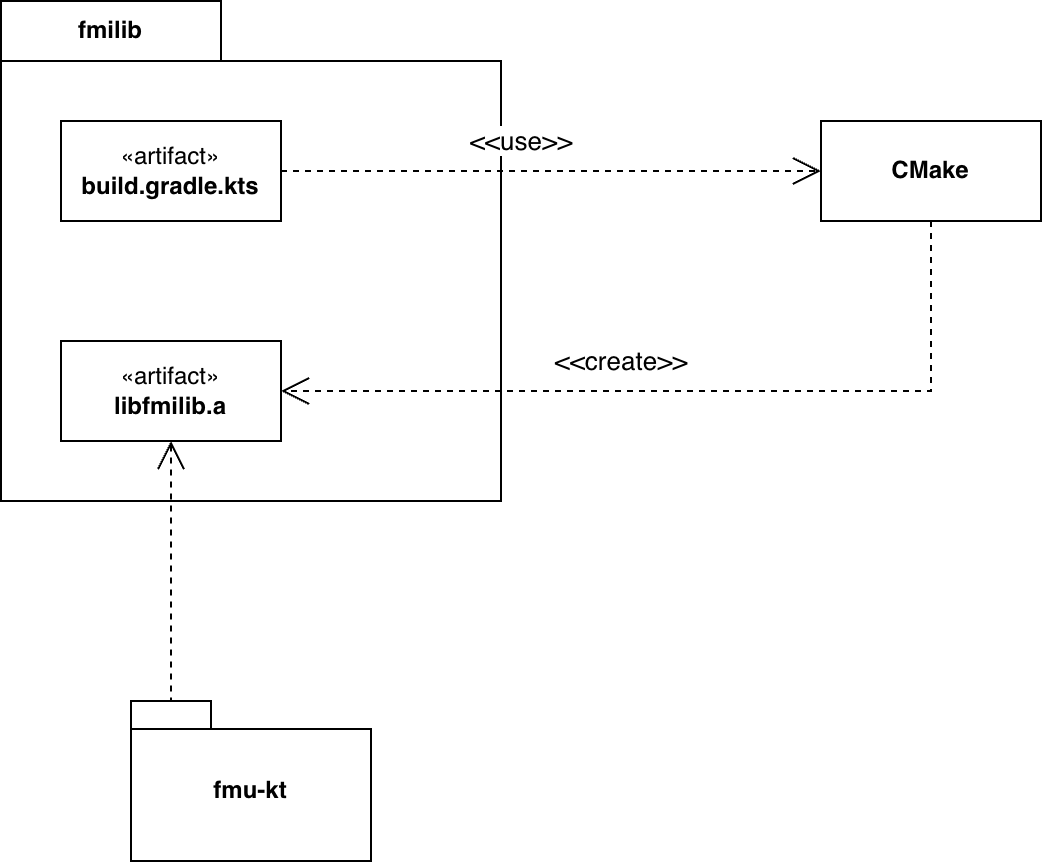
\includegraphics[width=0.54\textwidth]{images/diagramma-compilazione.png}
      \caption{Come avviene l'integrazione con il codice nativo.}
      \label{fig:nativo}
  \end{figure}
  \end{center}
\end{frame}


% ============================================================
\section{Supporto sperimentale a sistemi Apple Silicon}
% ============================================================

\begin{frame}{Supporto sperimentale a sistemi Apple Silicon}
  \begin{columns}
    \column{0.42\textwidth}
      \begin{itemize}
        \item FMU spesso solo in \texttt{x86\_64}, incompatibili con Apple Silicon
        \item Rosetta 2 non utilizzabile (caricamento dinamico via \texttt{dlopen})
      \end{itemize}
      % \begin{alertblock}{La domanda}
      %   Il monolinguaggio regge anche qui?
      % \end{alertblock}
    \column{0.55\textwidth}
      \begin{center}
      \begin{tikzpicture}[
        box/.style={draw=thesisBlue, fill=thesisBg, rounded corners=2pt,
                    minimum width=2.6cm, minimum height=0.7cm,
                    font=\scriptsize, align=center},
        arch/.style={box, fill=thesisBlue!10},
        result/.style={box, fill=thesisBlue!25, font=\scriptsize\bfseries},
        arrow/.style={->, thick, color=thesisBlue},
        node distance=0.6cm and 1.4cm,
      ]
        % Sorgente
        \node[box] (src) {Sorgenti C modello\\\texttt{sources/}};
        % Due compilazioni parallele
        \node[arch, below left=0.9cm and 0.4cm of src] (x86)
          {Compilazione\\\texttt{-arch x86\_64}};
        \node[arch, below right=0.9cm and 0.4cm of src] (arm)
          {Compilazione\\\texttt{-arch arm64}};
        % lipo: ben più in basso del bordo inferiore di x86/arm
        \node[box, below=2.2cm of src, fill=thesisGray!15] (lipo)
          {\texttt{lipo}};
        % Fat binary risultante
        \node[result, below=0.7cm of lipo] (fat)
          {Fat binary\\universale (\texttt{.dylib})};
        % Frecce: scendono prima, poi vanno verso lipo.north
        \draw[arrow] (src.south) -- ++(0,-0.2) -| (x86.north);
        \draw[arrow] (src.south) -- ++(0,-0.2) -| (arm.north);
        \draw[arrow] (x86.south) -- ++(0,-0.2) -| (lipo.north);
        \draw[arrow] (arm.south) -- ++(0,-0.2) -| (lipo.north);
        \draw[arrow] (lipo.south) -- (fat.north);
      \end{tikzpicture}
      \end{center}
  \end{columns}
\end{frame}


% % ============================================================
% \section{Demo}
% % ============================================================

% \begin{frame}{Demo dal vivo}
%   \centering
%   \Large Dimostrazione pratica dell'applicativo
% \end{frame}


% ============================================================
\section{Valutazione}
% ============================================================

\begin{frame}{Valutazione}
  \begin{columns}
    \column{0.55\textwidth}
      \begin{itemize}
        \item Test unitari dei moduli
        \item Test di integrazione su FMU pubblici (submodule git + Kotest)
        \item CI su GitHub Actions: Windows, Linux, macOS
      \end{itemize}
    \column{0.4\textwidth}
      \begin{block}{Sintesi}
        Sistema validato, non solo compilato, su tutte le piattaforme target
      \end{block}
  \end{columns}
\end{frame}


% ============================================================
\section{Conclusioni e sviluppi futuri}
% ============================================================

\begin{frame}{Conclusioni}
  \begin{columns}
    \column{0.48\textwidth}
      \begin{block}{Obiettivi raggiunti}
        \begin{itemize}
          \item Caricamento FMU (+ ricompilazione su macOS)
          \item Visualizzazione metadati e variabili
          \item Configurazione simulazione (variabili, durata, passo)
          \item Grafico dei risultati
        \end{itemize}
      \end{block}
    \column{0.48\textwidth}
      \begin{alertblock}{Limitazioni}
        \begin{itemize}
            \item Solo standard FMI 2.0
            \item Ricompilazione macOS: soluzione best-effort
            \item Kotlin/Native: stdlib limitata, più lavoro manuale (es. API POSIX)
        \end{itemize}
      \end{alertblock}
  \end{columns}
\end{frame}


% ── IMMAGINI ─────────────────────────────────────────────
\begin{frame}{Conclusioni}
    \begin{columns}
        \column{0.48\textwidth}
            \begin{figure}
              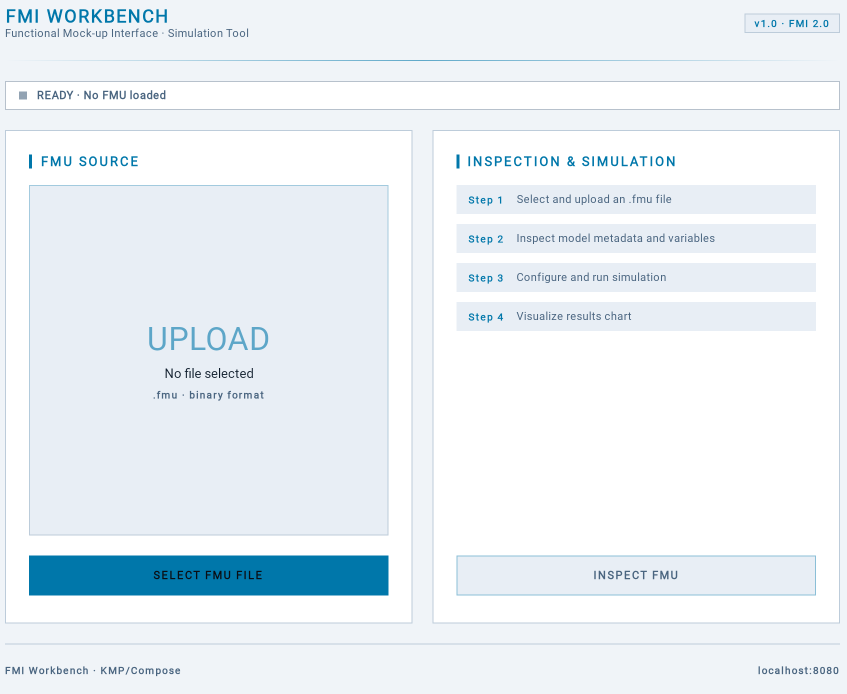
\includegraphics[width=\textwidth]{images/home-screen.png}
              \caption{Schermata di upload.}
              \label{fig:home}
            \end{figure}
        \column{0.48\textwidth}
            \begin{figure}
              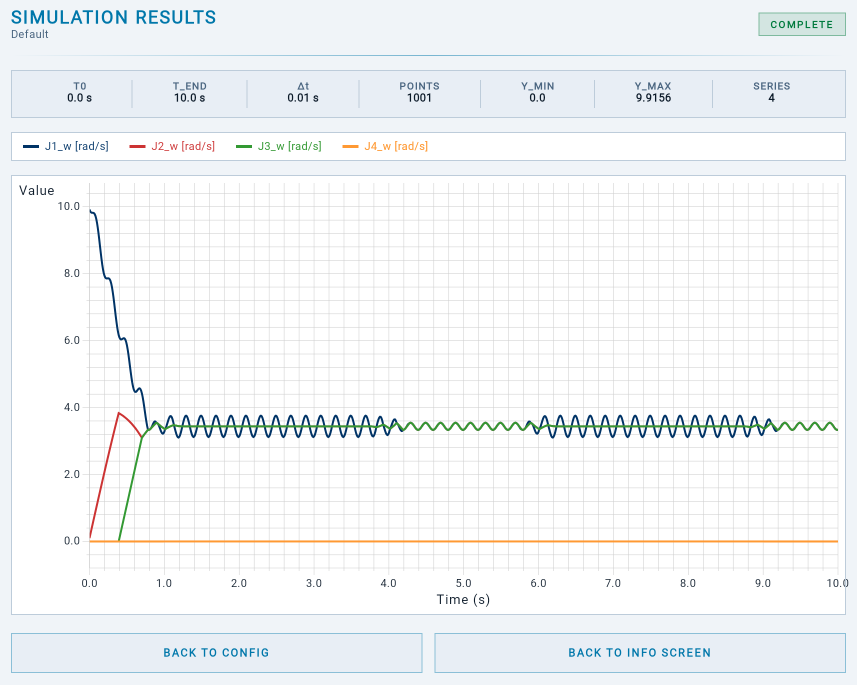
\includegraphics[width=\textwidth]{images/chart-screen.png}
              \caption{Grafico di una simulazione.}
              \label{fig:chart}
        \end{figure}
    \end{columns}
\end{frame}

% ── SVILUPPI FUTURI ─────────────────────────────────────────────
\begin{frame}{Conclusioni}
        \centering
        \begin{block}{Sviluppi futuri}
            \begin{itemize}
                \item Supporto ad altre versioni dello standard FMI
                \item Esportazione dei risultati della simulazione
                \item Gestione di più modelli FMU in contemporanea
            \end{itemize}
        \end{block}
\end{frame}

% ── SLIDE FINALE ─────────────────────────────────────────────
\begin{frame}
  \centering
  \Large Grazie per l'attenzione\\[0.5em]
\end{frame}

\end{document}